\chapter{Uncertainty quantification in geometry reconstruction} \label{ch:uncertainty}

\vspace{-1.5 em}
\begin{addmargin}[-0.5cm]{0cm}
  \minitoc
\end{addmargin}
\hrule
\vspace{1.5 em}

In the previous two chapters, we approached the task of geometry reconstruction using two approaches, a lookup table which was only feasible for the reconstruction of triatomic molecules, and the more sophisticated optimization approach. We also ended on a rather troubling note regarding the feasibility of geometry reconstruct, namely that the reconstructed geometries exhibited unusual bond length correlations (section \ref{ssec:weirdBonds}) and that degenerate geometries can be found in large region of phase space (section \ref{sec:optimizationDegeneracies}).

In this chapter we will begin by tackling the important task of quantifying the uncertainty on our geometry reconstructions, which surprisingly has not been performed by any previous study. We will take a heuristic approach, which provides some valuble estimates on the amount of uncertainty to expect and will help resolve the issue of unusual bond length correlations. A more rigorous and sophisticated approach of uncertainty quantification in the Bayesian inference framework was attempted and although it has stagnated, the motivation and methodology of this approach will be discussed.

\section{Uncertainty on a reconstructed geometry} \label{sec:heuristicApproach}
The question of interest in this section is, \textit{``how does uncertainty in the measured momentum vectors affect the uncertainty of the reconstructed geometry?''} We have already calculated the uncertainty on the momentum vectors in section \ref{ssec:measurementUncertainty} but we cannot derive an analytic formula for the uncertainty on the molecular parameters or the atomic positions.

\subsection{A heuristic approach}
We will take a very basic approach here by attempting to generalize a simple result for the propagation of error through a monotonically increasing function. A monotonically increasing function is always increasing, that is, it always has a positive first derivative.

If a particular measurement $\bar{x}$ of a variable $x$ carries some uncertainty $\epsilon$ such that the true value of $\bar{x}$ lies within some interval $\bar{x} - \epsilon \le \bar{x} \le \bar{x} + \epsilon$ then the true value of some arbitrary monotonically increasing scalar function $f(x)$ that is dependent on the value of the measurement will lie within some interval
\begin{equation}
  f(\bar{x} - \epsilon) \le f(\bar{x}) \le f(\bar{x} + \epsilon)
\end{equation}

Now if we relax the condition that $f$ be a monotonically increasing function, then the true value of $f(\bar{x})$ can take on any value that $f$ attains within the interval $\bar{x} - \epsilon \le \bar{x} \le \bar{x} + \epsilon$, and we can say very generally that it lies between
\begin{equation} \label{eq:shittyInterval}
  \min_{\displaystyle \bar{x} - \epsilon \le x \le \bar{x} + \epsilon} \; f(x)
  \le f(\bar{x})
  \le \max_{\displaystyle \bar{x} - \epsilon \le x \le \bar{x} + \epsilon} \; f(x)
\end{equation}
which however, may not yield a useful interval, especially in the presence of discontinuities or divergences. However, for finite-valued and well-behaved functions that do not change rapidly within the interval $\bar{x} - \epsilon \le \bar{x} \le \bar{x} + \epsilon$, \eqref{eq:shittyInterval} may provide a useful upper bound on the uncertainty in $f(\bar{x})$. This could be particularly accurate for small neighbourhoods about $\bar{x}$. As geometry reconstruction produces physically reasonable values for the molecular parameters without any discontinuties or divergences, we will attempt to use this idea to quantify the uncertainty on a geometry's reconstruction.

Before generalizing these two ideas for multivariable measurements and functions, it will be helpful to look at this idea for the case of measurement of a vector of two variables $\bar{\mathbf{x}} = (\bar{x}_1, \bar{x}_2)$ with an uncertainty described by the vector $\bm{\epsilon} = (\epsilon_1, \epsilon_2)$ and error propagation through a vector-valued function of two variables $\mathbf{f}(\mathbf{x}) = (f_1(\mathbf{x}), f_2(\mathbf{x}))$. We will treat $\mathbf{f}(\mathbf{x})$ as non-parametric and assume that it has no analytic form, \ie~ as a \emph{black box} function as the mapping from momentum vector measurements to geometries cannot be parameterized or given in any analytical form.

In this case the true value of $\bar{\mathbf{x}}$ lies within a box described by $\bar{x}_1 - \epsilon_1 \le \bar{x}_1 \le \bar{x}_1 + \epsilon_1$ and $\bar{x}_2 - \epsilon_2 \le \bar{x}_2 \le \bar{x}_2 + \epsilon_2$ in the $x_1x_2$ plane. If both $f_1(\mathbf{x})$ and $f_2(\mathbf{x})$ depend monotonically on $x_1$ and $x_2$ then determining the range of possible values of $\mathbf{f}(\bar{x})$ would be simple. Evaluating $\mathbf{f}(\mathbf{x})$ for 
\begin{equation} \label{eq:endpoints}
\mathbf{x} \in \mathbf{x}_\mathrm{ep}
  % = \lbrace (\bar{x}_1 \pm \epsilon_1, \bar{x}_2 \pm \epsilon_2) \rbrace
  = \left\lbrace
    \begin{pmatrix} x_1 - \epsilon_1 \\ x_2 - \epsilon_2 \end{pmatrix},
    \begin{pmatrix} x_1 - \epsilon_1 \\ x_2 + \epsilon_2 \end{pmatrix},
    \begin{pmatrix} x_1 + \epsilon_1 \\ x_2 - \epsilon_2 \end{pmatrix},
    \begin{pmatrix} x_1 + \epsilon_1 \\ x_2 + \epsilon_2 \end{pmatrix}
  \right\rbrace
\end{equation}
where $\mathrm{ep}$ is an abbreviation for ``endpoints'' (as $\mathbf{x}_\mathrm{ep}$ denotes the set of endpoints for the box containing feasible values of $\mathbf{x}$ in the $x_1x_2$ plane) would produce $4$ point in the $f_1f_2$ plane, whose set we denote by $\mathbf{f}_\mathrm{ep}$ and whose rectangular boundary encloses the possible values of $f(\bar{x})$. Thus the propagation of uncertainty in this case can be thought of a mapping from a rectangle in the $x_1x_2$ plane to a rectangle in the $f_1f_2$ plane.

If $f_1$ and $f_2$ do not depend monotonically on $x_1$ and $x_2$, then values of $x_1$, $x_2$ between the endpoints may produce values of $f_1$,$f_2$ that lie outside the rectangular boundary. A further heuristic would be to not only look at the endpoints, but also a set of uniformally distributed points in the $x_1x_2$ plane within the box of possible values for $\mathbf{x}$. In this case, the propagation of uncertainty can be thought of as a mapping from a rectangle in the $x_1x_2$ plane to an arbitrary region in the $f_1f_2$ plane whose boundary may not be rectangular anymore, or even a single region. In the case of a more complicated boundary, we will generalize \eqref{eq:shittyInterval} by describing the boundary using a \emph{convex hull}. The convex hull $C$ of a set of points $S = \lbrace p_1, p_2, \dots, p_n \rbrace$ where $p_i \in \mathbb{R}^m$ for all $i$ can be expressd mathematically as
\begin{equation} \label{eq:convexhull}
C = \left\lbrace\left.
  \sum_{i=1}^n \lambda_i p_i \right|
  \lambda_i \ge 0
  \;\; \mathrm{and} \;\;
  \sum_{i=1}^n \lambda_i = 1
  \right\rbrace
\end{equation}
An analogy in two dimensions would be to stretch a rubber band around the set of points and let it rest, its final shape being the convex hull.

%by the set of convex combinations of the points in $\mathbf{f}_\mathrm{ep}$,
%\begin{equation}
%  \displaystyle
%  \left\lbrace\left.
%  \sum_{\mathbf{f} \in \mathbf{f_i}_\mathrm{ep}}^{|\mathbf{f}_\mathrm{ep}|}
%  \alpha_i\mathbf{f_i}
%  \right| \alpha_i \ge 0 \; \mathrm{and} \;
%  \sum_i^{|\mathbf{f}_\mathrm{ep}|} \alpha_i = 1
%  \right\rbrace
%\end{equation}
%which is the convex hull of the set of points contained in $\mathbf{f}_\mathrm{ep}$, discussed further in the next subsection.

Extending this idea to our problem of geometry reconstruction, we have $9$ measurements $\bar{\mathbf{p}} = (\bar{p}_1, \dots, \bar{p}_9)$ with uncertainty $\bm{\epsilon} = (\epsilon_1, \dots, \epsilon_9)$ and we are interested in the range of possible geometries as produced by $\mathbf{g}(\mathbf{p}) = (r_{12}(\mathbf{p}), r_{23}(\mathbf{p}), \theta(\mathbf{p}))$. The possible values of the momentum components are contained within a $9$-dimensional hyperrectangle or box in momentum space, and we would like to obtain a $3$-dimensional region in phase space describing the set of possible geometries that the measurement could correspond to. Generating a set of $N$ uniformally distributed points within the $9$-dimensional box would produce $N^9$ sets of momentum vectors, each of which must be reconstructed. This represents a rather unfeasible number of reconstructions to perform, thus we will start by looking at the set of endpoints only, which contains $512$ ($2^9$) sets of momentum vectors. Attempting to reconstruct a geometry for each set of momentum vectors will ideally provide us with $512$ geometries that together give us some idea into the range of possible geometries the measurement could possibly belong to. By only reconstructing the endpoints of our box in momentum space, we may be underestimating the range of possible geometries as points within the box may produce more extreme geometries when reconstructed.

% % r_CO=131.677 pm, r_CS=187.161 pm, theta=169.42 deg
To carry out this idea for geometry reconstruction, we randomly chose a representative geometry, $(r_\mathrm{CO}, r_\mathrm{CS}, \theta) = (\SI{130}{\pico\m}, \SI{190}{\pico\m}, \SI{169}{\degree})$ that does not lie in any of the degenerate regions discussed in figure \ref{fig:OCS222DegeneracyMaps} to avoid having to account for degenerate geometries. Simulating a Coulomb explosion using this geometry as the intial condition yields a set of momentum vectors, upon which we artifically placed an uncertainty of $5\%$ for each momentum component such that $\bm{\epsilon} = 0.05\mathbf{p}$, producing $512$ sets of momentum vectors corresponding to the corners of the $9$-dimensional box in momentum space, that is, a 9-dimensional version of \eqref{eq:endpoints}. Reconstructing a geometry for each set of momentum vectors, we obtain $512$ geometries and all $512$ sets of momentum vectors were successfully mapped to a unique geometry. Histograms showcasing the bond length and bond angle distributions of these reconstructed geometries are plotted in figure \ref{fig:OCS222Uncertainty} along with scatter plots showcasing the bivariate relationships between the three molecular parameters.

\begin{figure}
  \centering
  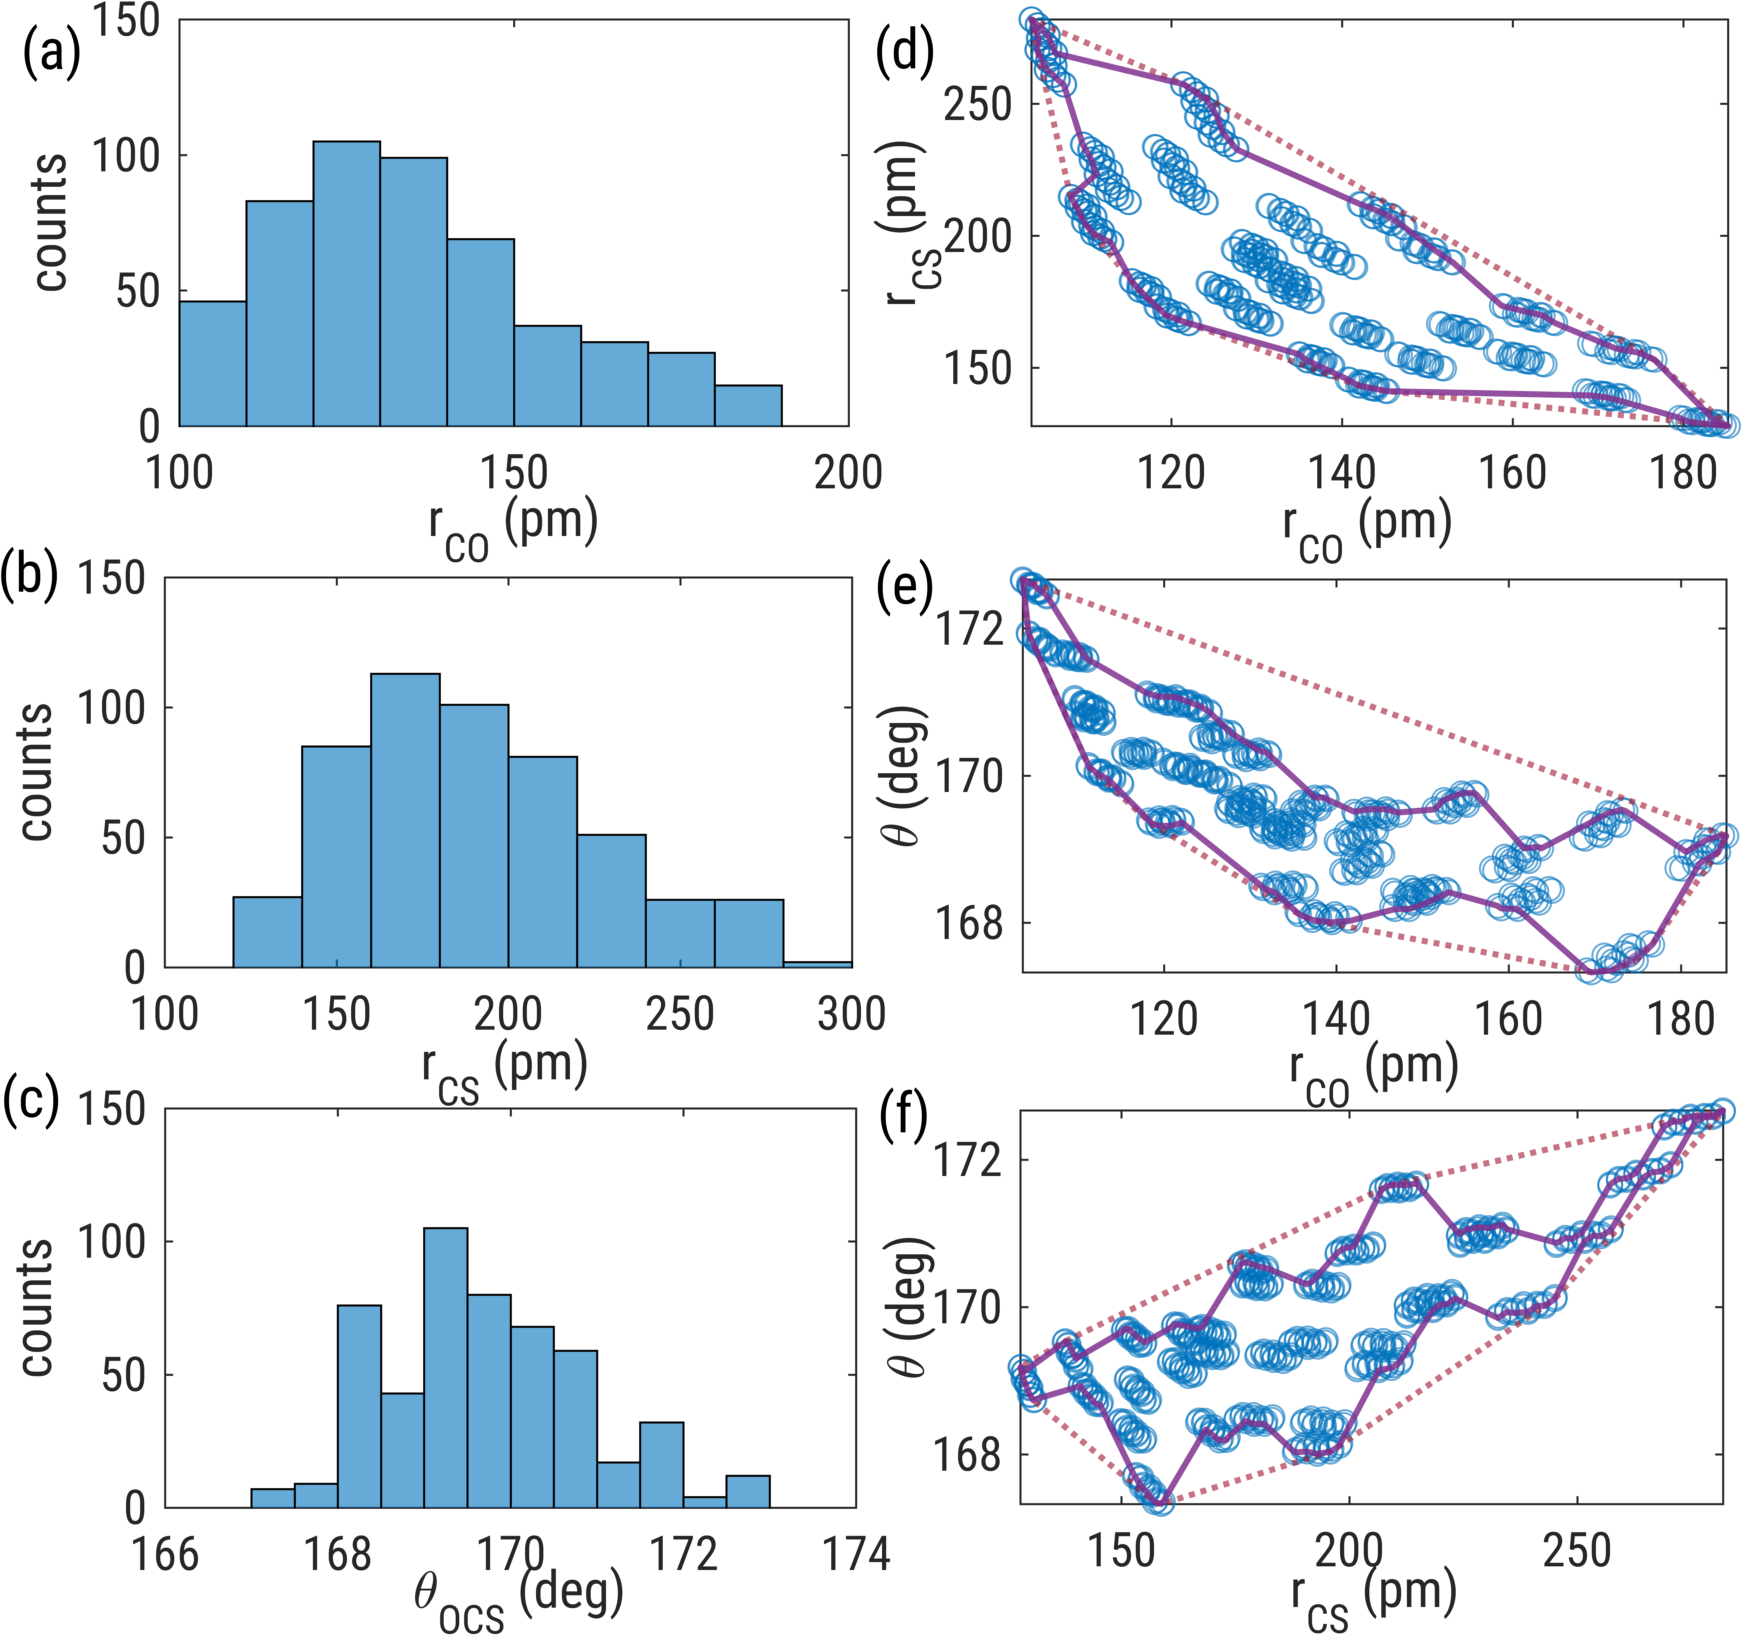
\includegraphics[width=\textwidth]{Plots/OCS222Exploration1_5percent}
  \caption[A heuristic estimate on the range of possible \ch{OCS} $(2,2,2)$ geometries that may be reconstructed assuming a true geometry of $(r_\mathrm{CO}, r_\mathrm{CS}, \theta) = (\SI{130}{\pico\m}, \SI{190}{\pico\m}, \SI{169}{\degree})$ and $5\%$ uncertainty on the measured momentum vectors.]
  {A heuristic estimate on the range of possible \ch{OCS} $(2,2,2)$ geometries that may be reconstructed assuming a true geometry of $(r_\mathrm{CO}, r_\mathrm{CS}, \theta) = (\SI{130}{\pico\m}, \SI{190}{\pico\m}, \SI{169}{\degree})$ and $5\%$ uncertainty on the measured momentum vectors. Histograms showcase the (a) \ch{C-O} bond length, (b) \ch{C-S} bond length, and (c) bond angle distributions of the reconstructed geometries. Scatter plots showcase the bivariate relationships between (d) $r_\mathrm{CO}$ and $r_\mathrm{CS}$, (e) between $r_\mathrm{CO}$ and $\theta$, and (f) between $r_\mathrm{CS}$ and $\theta$. Each reconstructed geometry is plotted as an open blue circle. The boundary of the set of reconstructed geometries is calculated using two methods and plotted; The dotted red line denotes the convex hull and the solid purple line denotes the alpha shape (using (d) $\alpha=15$, (e) $\alpha=22$, and (f) $\alpha=30$) of the set of points.}
  \label{fig:OCS222Uncertainty}
\end{figure}

We immediately see that a strikingly wide range of geometries are reconstructed assuming the momentum components carry an uncertainty of only $5\%$. Inspection suggests that the bond length and bond angle distributions roughly form a Gaussian distribution about the true parameters. The distributions encompass a wide range of possible bond lengths, \SI{80}{\pico\m} for the \ch{C-O} bond and \SI{175}{\pico\m} for the \ch{C-S} bond. The variability in the bond angle is not as extreme, encompassing a \SI{6}{\degree} range of possible bond angles.

The bivariate relationships shown in figures \ref{fig:OCS222Uncertainty}(d)-(f) suggest the range of possible geometries. Interestingly, the bond length correlation in figure \ref{fig:OCS222Uncertainty}(d) seems to follow a reciprocal relationship, a strikingly similar one to the unusual one observed in the reconstructions of experimental data. This suggests that uncertainty in the momentum measurments may lead to the reconstruction of a geometry with asymetrically stretched bonds, and that the unusual relationship we observed in section \ref{ssec:weirdBonds} may have been a manifestation of measurement uncertainty and due to the highly sensitive nature of geometry reconstruction.

Placing a larger uncertainty on the momentum vector components further stretches the shape of the set of points in figure \ref{fig:OCS222Uncertainty}(d), modifying it to further resemble the more extreme reciprocal relationship between $r_\mathrm{CO}$ and $r_\mathrm{CS}$ found for longer pulse lengths (see figures \ref{fig:OCS22230fsMOGeometryPairs} -- \ref{fig:OCS222100fsMOGeometryPairs}). 

Exposing the molecule to longer laser pulses provides a longer amount of time for the molecule to rearrange and may impart the atomic fragments with a larger initial momentum, thus decreasing the certainty with which the measured momentum vectors correspond to the true geometry. If we take a reciprocal relationship to be a signature indicating that too much measurement uncertainty is present for trustworthy geometry reconstructions, then we must conclude that even an uncertainty as low as a few parts per hundred in the momentum vector components is ``too much'' and that geometry reconstruction using Coulomb explosion imaging is unfeasible under such conditions.

We may use the area formed by the set of points in figures \ref{fig:OCS222Uncertainty}(d)-(f), plotted as red dotted lines by the use of a convex hull, as a quantitative measure of uncertainty. Another boundary may be provided by the \emph{alpha shape} of the set of points, plotted as solid purple lines.

An interesting observation resulting from the close inspection of the open blue circles in figures \ref{fig:OCS222Uncertainty}(d)-(f) is the clustering of geometries in phase space as geometries seem to cluster in little groups. Each geometry is actually paired with one other geometry (close inspection of the open blue circles should reveal that they appear in pairs, sometimes appearing as a single blurred circle) so that $256$ points are visible unless the scatter plots are very closely inspected. As we picked one of two extreme values, $\bar{p} - \epsilon$ and $\bar{p} + \epsilon$ for each momentum component, each component may be responsible for the ``splitting of the geometries'' into pairs or clusters. This suggests that some uncertainty in certain momentum components may have a greater effect on the uncertainty of reconstructed geometries.

\subsection{Convex hulls and alpha shapes}
To quantify the uncertainty in the geometries, we will use two useful concepts from computational geometry, namely convex hulls and alpha shapes, which allow us to assign a shape and a volume to a set of points, and thus provide an additional hueristic quantitative measure of uncertainty.

The convex hull of a set of points, introduced earlier and described mathematically by \eqref{eq:convexhull}, is used to assign boundaries in phase space for figures \ref{fig:OCS222Uncertainty}(d)-(f). Many algorithms exist to calculate the convex hull, especially in 2 or 3 dimensions. However, the convex hull may grossly overestimate the area especially 

The concept of an alpha shape is a generalization of the convex hull used to assign shapes and volumes to a set of points, parameterized by a real number $\alpha \ge 0$. $\alpha$ may be varied until a desired shape is produced. They were first introduced by \citet{Edelsbrunner83} for two-dimensional shapes, then for three-dimensional shapes \citep{Edelsbrunner94} with applications in fields such as computer graphics. Interestingly, alpha shapes have been used to analytically compute shapes for macromolecules such proteins and estimate their molecular areas and volume \citep{Liang98}. % An interesting analogy of alpha shapes uses ice cream scoopers.

A desirable feature of convex hulls is that they are unique for each set of points, while multiple distinct alpha shapes exist. This is a desirable property of alpha shapes as there is no formal concept of shape so no algorithm can determine the correct shape for a set of points. However, the concept allows for an $\alpha$ to be picked that produces the most desirable shape. 

While a very haphazard measure of uncertainty, they are much easier to employ than the sophisticated uncertainty quantification framework of Bayesian inference and satisfy our basic needs for now.

% We end by providing a cool figure showcasing the three-dimensional convex hull and alpha shape in molecular phase space.

% figure Z here

\section{Determining the sources of uncertainty} \label{sec:sourceUncertainty}
We saw in figures \ref{fig:OCS222Uncertainty} that certain momentum components may have a greater effect on the uncertainty on a reconstructed geometry, or that geometry reconstruction is more sensitive to changes in certain momentum components over others.

We will attempt to explore this effect and pinpoint the momentum components responsible for introducing the most (and the least) uncertainty in the reconstructed geometries. To do this for the oxygen's $p_x$ component for example, we will look at the $256$ geometries reconstructed using the $256$ sets of momentum vectors where $5\%$ was added to the oxygen's $p_x$ component, and plot their position in phase space in the $r_\mathrm{CO}r_\mathrm{CS}$ plane. Doing this for each component, we produce $9$ plots in total, one for each momentum component, as shown in figure \ref{fig:OCS222DeterminingSource}.

\begin{figure}
  \centering
  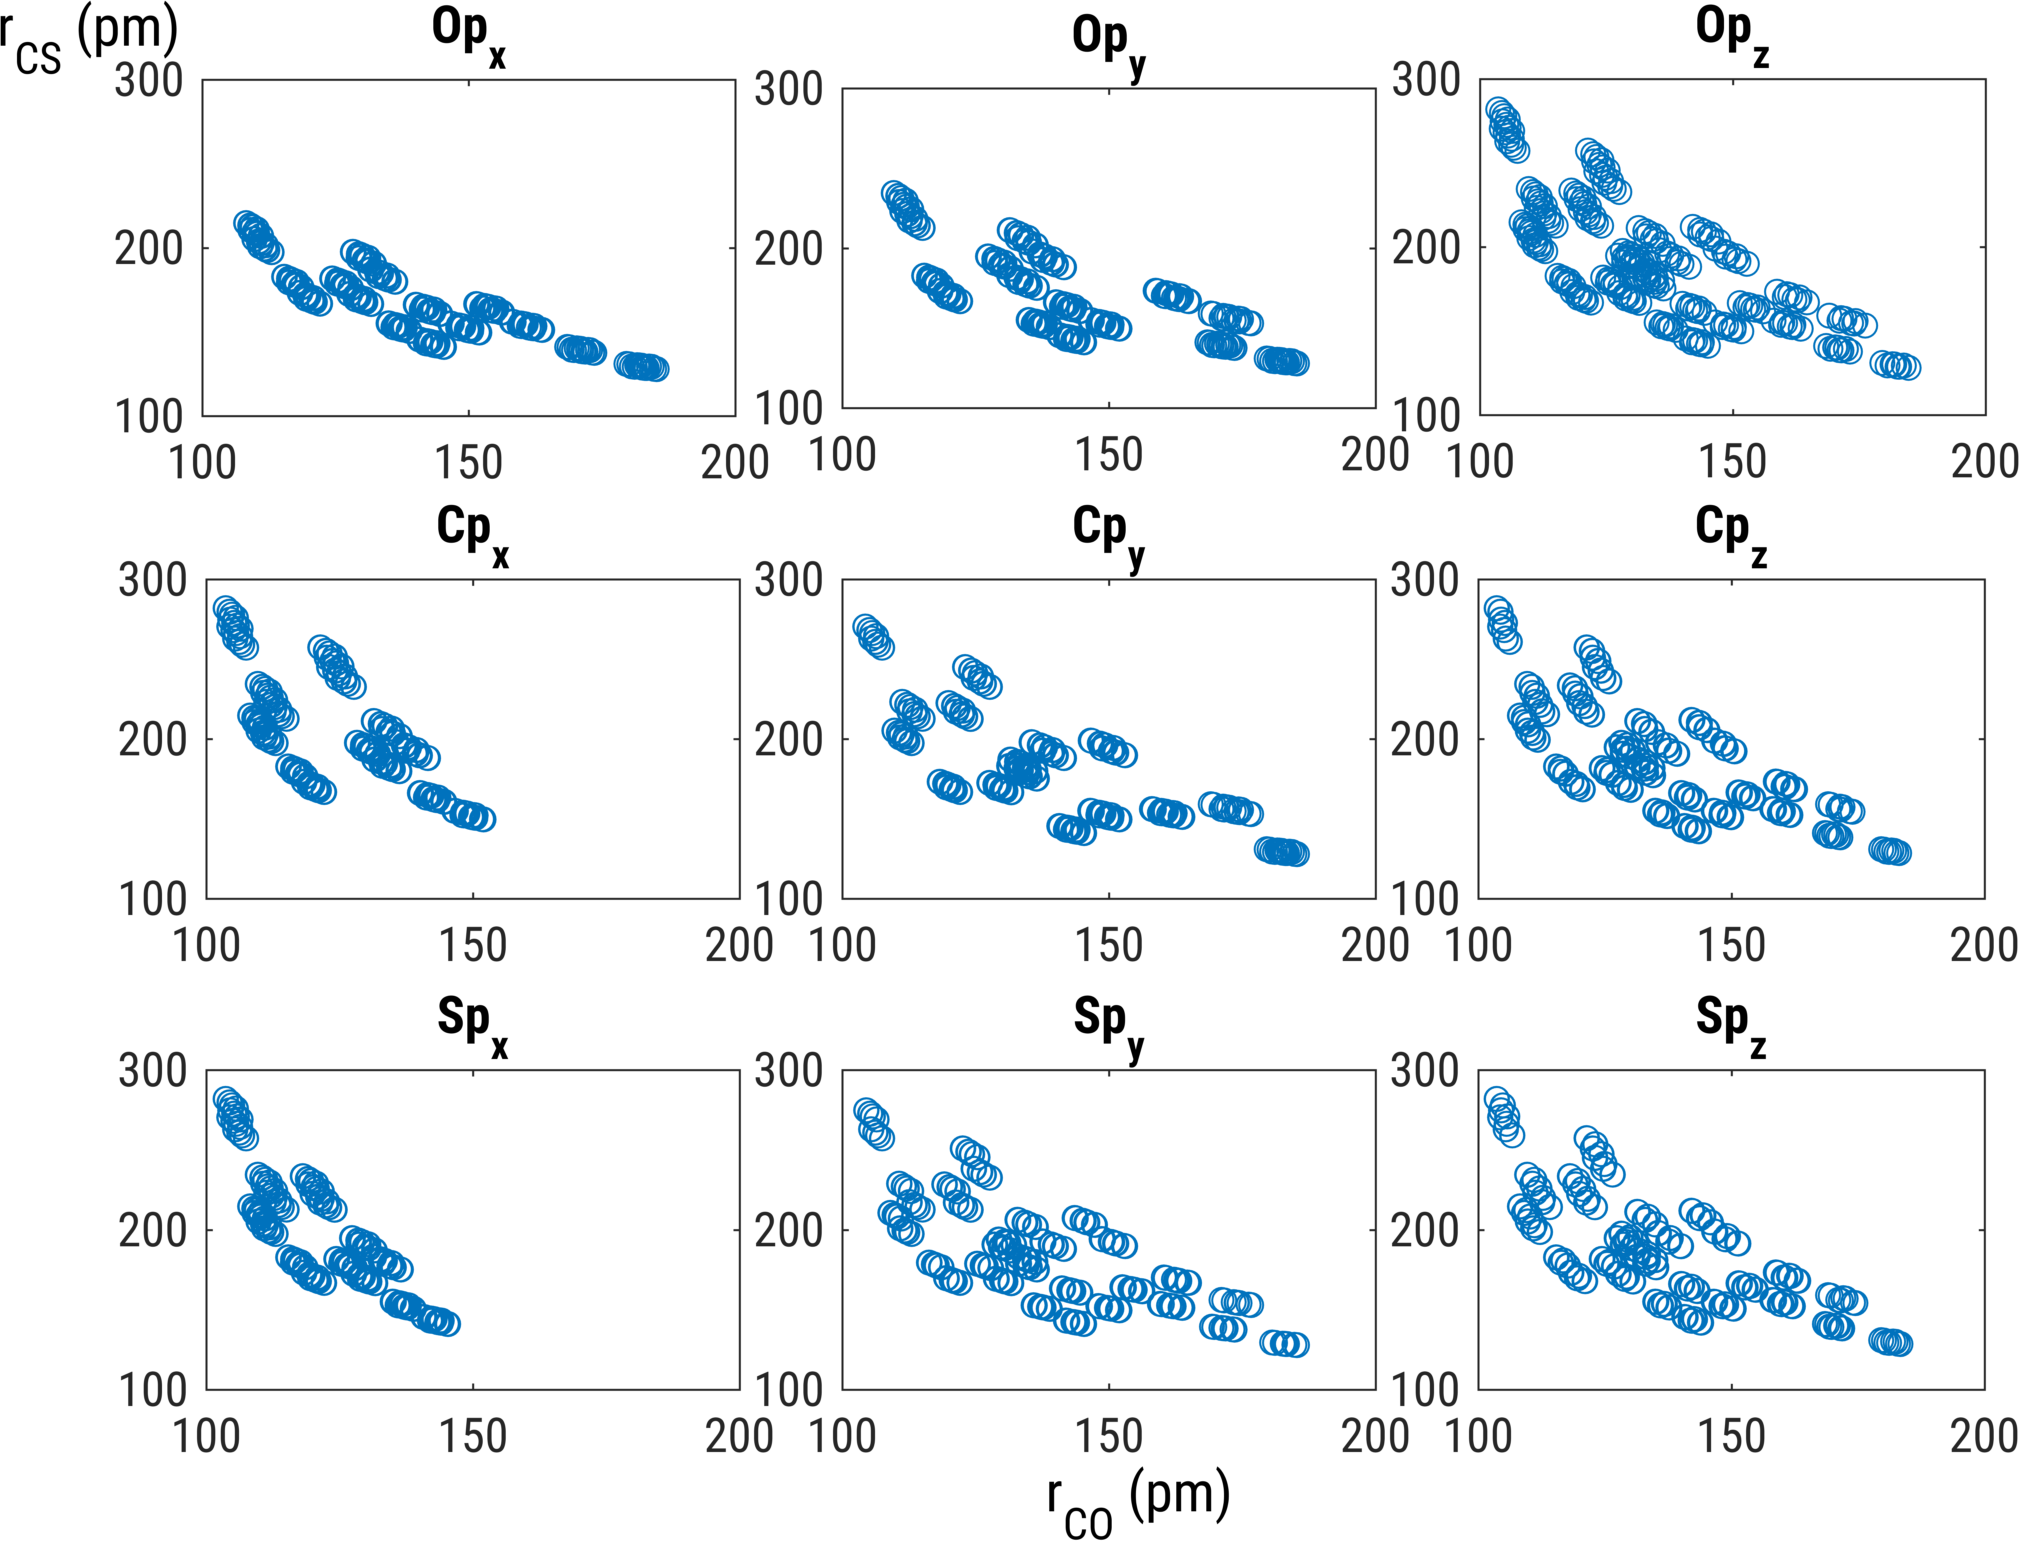
\includegraphics[width=\textwidth]{Plots/OCS222Exploration2}
  \caption[Scatter plots providing a heuristic estimate on the range of possible \ch{OCS} $(2,2,2)$ geometries that may be reconstructed assuming a true geometry of $(r_\mathrm{CO}, r_\mathrm{CS}, \theta) = (\SI{130}{\pico\m}, \SI{190}{\pico\m}, \SI{169}{\degree})$ and $5\%$ uncertainty on the measured momentum vector components except for the single component indicated in the title of each scatter plot.]
  {Scatter plots providing a heuristic estimate on the range of possible \ch{OCS} $(2,2,2)$ geometries that may be reconstructed assuming a true geometry of $(r_\mathrm{CO}, r_\mathrm{CS}, \theta) = (\SI{130}{\pico\m}, \SI{190}{\pico\m}, \SI{169}{\degree})$ and $5\%$ uncertainty on the measured momentum vector components except for the single component indicated in the title of each scatter plot. For each plot the \ch{C-O} bond length is plotted on the horizontal axis and the \ch{C-S} bond length on the vertical axis.}
  \label{fig:OCS222DeterminingSource}
\end{figure}

We immediately see that some momentum components are responsible for larger variations in the reconstructed geometries than others. The carbon and sulfur's $p_x$ components seem responsible for almost doubling the variability in the \ch{C-O} bond length while the oxygen's $p_x$ component seems responsible for almost doubling the variability in the \ch{C-S} bond length. Very close inspection reveals that removing the uncertainty on the oxygen's $p_z$ component removes the pairing up of the geometries, suggesting that uncertainty on oxygen's $p_z$ component is largely irrelevant for geometry reconstruction.

The exact dependence observed in figure \ref{fig:OCS222Uncertainty}, that is, which components contribute more to the uncertainty of reconstructed geometries, may be due to experimental setup factors such as the polarization of the laser's electric field or the initial orientation of the molecule at the start of the Coulomb explosion. It may also depend on the convention used to rotate and describe the momentum vectors (section \ref{sec:conventions}).

Further investigation is certainly warranted, especially if one aims to design a Coulomb explosion imaging experiment for the purposes of minimizing errors in geometry reconstruction. Molecules may be oriented to minimize errors in geometry reconstruction, for example.

\section{Exploratory uncertainty analysis} \label{sec:uncertaintyAnalysis}
Our main intentions in this chapter were twofold. Firstly, to suggest that measurement uncertainty is responsible for the asymmetric bond length correlations that arise out of both reconstruction methods, and secondly, to suggest that uncertainty on certain momentum components results in a larger error on the reconstructed geometries which, upon further investigation, may be exploited in the design of CEI experiments for minimizing errors in geometry reconstruction.

In this section we will simply describe some further investigations or rather, \emph{explorations}, that may be carried out to study the effects of measurement uncertainty on the geometry reconstruction process.

A major drawback to the analysis performed in section \ref{sec:heuristicApproach} is the large number of geometries that must be reconstructed, $2^9$ for a triatomic molecule if only the endpoints of the box in momentum space are used. For a molecule with $N$ atoms, this scales exponentially as $2^{3N}$. To reduce the number of reconstructions that must be performed, a simplified version of the analysis in section \ref{sec:sourceUncertainty} may be performed first. By adding uncertainty on each component one-by-one, $2\times3N$ different sets of momentum vectors are produced which may quickly reconstructed, hinting at which momentum components produce large errors in the reconstructed geometries, and which do not. The components that do not introduce large errors may be ignored when constructing the $3N$-dimensional box in momentum space, reducing the number of geometries to be reconstructed by a factor of $2$ for each component that introduces very small errors.

In using a convex hull or alpha shape to describe the set of possible geometries, we are neglecting that certain regions of phase space may contain a higher density of geometries than others. Thus, while the region may be quite large by itself, the vast majority of reconstructed geometries may lie within a smaller region of phase space. To determine the density of reconstructed geometries in phase space, momentum values lying between the end points must be reconstructed as well. This may be quite time-consuming to perfom and may require the reconstruction of many more than $2^{3N}$ geometries but may shed further insight. It will also be different for each measurement and thus, cannot be done for a data set consisting of hundreds of momentum vectors. A three-dimensional kernel density estimate may then provide an approximation to the probability distribution for the true geometry.

% Let's put a range of uncertainties on the momentum vectors and observe how much uncertainty we have on the reconstructed geometries. We will use the widths of the distributions and the convex hull and alpha shape areas and volumes to quantify the uncertainty with the aim of finding how uncertainty in geometry reconstruction varies as a function of uncertainty in the momentum vectors.

\section{Uncertainty quantification using Bayesian inference} \label{sec:uncertaintyBayesian}
The heuristic uncertainty quantification performed in the first two sections has provided significant insights on the process of geometry reconstruction, and emphasized the large effect that measurement uncertainty must have played in our reconstruction of experimental data. This further highlights the importance of tackling the task of uncertainty quantification in a rigorous and sophisticated manner, in which case the Bayesian inference framework provides a mature set of methods, software, and learning material to do this.

The Bayesian point of view provides a more natural and intuitive way of thinking about uncertainty in the physical sciences.

% Let us borrow an example from \citet{vanderPlas14}, who provides a primer comparing the frequentist and Bayesian approaches with several examples implemented in Python, to illustrate this point. Let us assume an astronomer is interested in measuring the photon flux $F$ of a star whose flux does not vary. Frequentist statistics defines the probability as a limiting case of repeated measurements and so after many repeated measurements, the true value of the flux $F$ is typically given as being within some \emph{confidence interval} with $95\%$ probability. Bayesian statistics 

The Bayesian approach allows us to write down the exact probability distribution we wish to find in terms of the measurements we have made and our prior beliefs and solve the resulting equations for it, such that our prior beliefs are updated based on the measurements we have made. Bayesian inference is also suitable for inferring unknown parameters in inverse problems.

Bayesian statistics actually predates the more commonly taught frequentist statistical methods (\eg~ p-values, confidence intervals, etc.) but has made a strong resurgence in recent years due to rising computational abilities and more recently, available software for parameter estimation in statistical models using Markov chain Monte Carlo methods \citep{Brooks03}. It is important to note that frequentist methods such as $t$-tests still have immense utility in the sciences, however, Bayesian inference methods provide the means of tackling more complex problems that are intractible otherwise. Bayesian methods have had large impacts in many scientific fields such as genetics \citep{Beaumont04} and more recently, machine learning \citep{Murphy12}, and an interpretation of quantum mechanics, termed \emph{Quantum Bayesianism}, exists as well \citep{Timpson08}. 

Many have argued for philosophical superiority of the Bayesian approach, most famously by \citet{Efron86} in his article titled ``\textit{Why isn't everyone a Bayesian?}''. \citet{Cousins95} authored a similarly titled article, ``\textit{Why isn't every physicist a Bayesian?}'' comparing both the classical and Bayesian frameworks in the context of particle physics. A more recent article on the subject authored by \citet{Lyons12} appeared in \emph{Physics Today}. Extensive review articles have been written on the general subject of Bayesian inference in physics and include numerous examples and case studies \citet{vonToussaint11,Dose03,Dagostini03}. Although not particularly writing about Bayesian inference, \citet{Hogg10} provide a rather excellent and extensive tutorial in fitting data to models in the form of an article, and include numerous excercises relying on the use of Bayesian inference.

Numerous textbooks exist on the topic. \citet{Gelman14} provide an excellent introduction to Bayesian data analysis, especially the theoretical foundations of Bayesian statistics, and \citet{Kruschke14} provides a practical and easy-to-follow introduction accompanied with many examples.

% 1. Setting up a full probability model—a joint probability distribution for all observable and unobservable quantities in a problem. The model should be consistent with knowledge about the underlying scientific problem and the data collection process.
% 2. Conditioning on observed data: calculating and interpreting the appropriate posterior distribution—the conditional probability distribution of the unobserved quantities of ultimate interest, given the observed data.
% 3. Evaluating the fit of the model and the implications of the resulting posterior distribution: how well does the model fit the data, are the substantive conclusions reasonable, and how sensitive are the results to the modeling assumptions in step 1? In response, one can alter or expand the model and repeat the three steps.

\subsection{Basic concept}
At the center of Bayesian statistics lies Bayes' theorem or Bayes' rule which describes the probability of an event based on prior knowledge of conditions that may be related to the event. It was first introduced by Reverend Thomas Bayes and published two years after his death with revisions by Ronald Price in a work titled ``\textit{An Essay towards solving a Problem in the Doctrine of Chances}'' \citep{Bayes1763} although evidence suggests that the title was modified by Price to support a theological arugment, and that Bayes intended it to be ``\textit{A Method of Calculating the Exact Probability of All Conclusions founded on Induction}'' \citep{Stigler13}. Pierre-Simon Laplace then developed it further and published it in its modern form along with many fundamental results in statistics \citep{Laplace1820}. \citet{Dale99} discusses the history in more detail, and \citet{McGrayne11} traces the history of Bayes' rule in her popular science book and its applications from World War II to bioinformatics.

Bayes' theorem in its simplest form states that probability of observing an event $A$ given that $B$ is true is
\begin{equation} \label{eq:BayesRule}
  P(A|B) = \frac{P(B|A) P(A)}{P(B)}
\end{equation}
where $P(B|A)$ is the probability that event $B$ occurs given that $A$ is true, and $P(A)$ and $P(B)$ are the probabilities that events $A$ and $B$ occur respectively. $P(A|B)$ denotes a conditional probability and can be expressed as $P(A|B) = P(A \cap B) / P(B)$ where $P(A \cap B)$ is the probability of both $A$ and $B$ occuring and $\cap$ denotes the intersection operation from set theory.\footnotemark~

\footnotetext{These concepts can all be made more rigorous in a modern framework. See \citet{Kallenberg06} for an introduction to modern probability theory.} 

For Bayesian inference of model parameters given that certain measurements or observations, the basic idea can be extracted from \eqref{eq:BayesRule}. Let us use $\theta$ to denote the parameters of a model, for example $\theta = (r_{12}, r_{23}, \phi)$ for a model of a triatomic molecule, and $y$ to denote data that has been measured or observed. We are interested in finding the \emph{posterior probability density} $P(\theta|y)$, the probability that our model is described by the parameters $\theta$ given that certain measurements $y$ have been made. Using \eqref{eq:BayesRule}, we can write
\begin{equation}
  P(\theta|y) = \frac{P(\theta) P(y|\theta)}{P(y)}
\end{equation}
where $P(\theta)$ denotes the \emph{prior distribution}, that is the probability distribution encapsulating our belief regarding the model parameters prior to making any measurements, and $P(y|\theta)$ is the \emph{likelihood function} is the distribution of observed data conditional on the model parameters. $P(y)$ is the \emph{marginal likelihood},
\begin{equation}
  P(y) = \int P(\theta) P(y|\theta) \mathop{d\theta}
\end{equation}
or the distribution of measurements marginalized over the model parameters. It can be difficult to compute as a high-dimensional integral. As it does not depend on $\theta$ it is a constant when considering a fixed set of measurements $y$, and thus we may instead be interested in computing the \emph{unormalized posterior density}
\begin{equation}
  \underbrace{P(\theta|y)}_\mathrm{posterior}
  \propto
  \underbrace{P(\theta)}_\mathrm{priot}
  \times
  \underbrace{P(y|\theta)}_\mathrm{likelihood}
\end{equation}

Using our geometry reconstruction problem for a triatomic molecule as an example, we are modeling a molecule using the parameters $\theta = (r_{12}, r_{23}, \phi)$ where $\phi$ now denotes the bond angle, and the measurements $y$ constitute a set of three momentum vectors $y = (\mathbf{p}_1, \mathbf{p}_2, \mathbf{p}_3)$ so \eqref{eq:BayesRule} gives
\begin{equation} \label{eq:BayesGeometry}
  P(r_{12}, r_{23}, \phi|\mathbf{p}_1, \mathbf{p}_2, \mathbf{p}_3) = \frac{P(\mathbf{p}_1, \mathbf{p}_2, \mathbf{p}_3|r_{12}, r_{23}, \phi) P(r_{12}, r_{23}, \phi)}{P(\mathbf{p}_1, \mathbf{p}_2, \mathbf{p}_3)}
\end{equation}
where $P(r_{12}, r_{23}, \phi)$ is the prior distribution and $P(\mathbf{p}_1, \mathbf{p}_2, \mathbf{p}_3|r_{12}, r_{23}, \phi)$ is the likelihood, that is the probability that the momentum vectors $(\mathbf{p}_1, \mathbf{p}_2, \mathbf{p}_3)$ are observed given that the molecule is described by the parameters $(r_{12}, r_{23}, \phi)$.

In our case, a uniform distribution or a guess distribution may be used for the prior, or it may be obtained from quantum chemicstry simulations for greater accuracy. Generally the posterior only depends strongly on the prior in the absence of sufficient data. \citet{Gelman14} discusses the choice of prior distribution in great detail. The likelihood function $P(\mathbf{p}_1, \mathbf{p}_2, \mathbf{p}_3|r_{12}, r_{23}, \phi)$ is governed by a deterministic simulation as exploding a certain molecule will produce exactly one set of momentum vectors, so in reality it is a Dirac-delta function. However, in the presence of measurement uncertainty it will form a proper probability distribution.

The denominator of \eqref{eq:BayesGeometry},
\begin{equation}
  P(\mathbf{p}_1, \mathbf{p}_2, \mathbf{p}_3) =
    \int P(\mathbf{p}_1, \mathbf{p}_2, \mathbf{p}_3|r_{12}, r_{23}, \phi)
    \mathop{dr_{12}} \mathop{dr_{23}} \mathop{d\phi}
\end{equation}
will be extremely difficult to calculate in general as it is the probability that the momentum vectors $(\mathbf{p}_1, \mathbf{p}_2, \mathbf{p}_3)$ are measured, regardless of the molecular geometry that produced them. As the marginal likelihood is simply a scaling factor, we will instead be interested in computing the unnormalized posterior density
\begin{equation}
  P(r_{12}, r_{23}, \phi|\mathbf{p}_1, \mathbf{p}_2, \mathbf{p}_3) \propto P(\mathbf{p}_1, \mathbf{p}_2, \mathbf{p}_3|r_{12}, r_{23}, \phi) P(r_{12}, r_{23}, \phi)
\end{equation}
Evaluating this expression can still be difficult, and the usual approach is to randomly sample from it, forming a posterior probability density in the process. \emph{Markov chain Monte Carlo} methods provide the means of doing this.

\subsection{Markov chain Monte Carlo}
% The basic idea
Performing the multi-dimensional integral can be very difficult. The integral is usually approximated using Markov Chain Monte Carlo.
% Markov Chain Monte Carlo: transition kernel, checking for convergence, Metropolis-Hastings algorithm, Gibbs Sampling, Hamiltonian MCMC

\citet{Diaconis09} gives a introduction to MCMC methods with a focus on their impact on the types of scientific and mathematical problems they have allowed us to solve, opening with a fascinating example of deciphering coded messages between prison inmates. \citet{Richey10} and \citet{Robert11} give a short history of MCMC methods and their development. 

An extensive handbook on MCMC methods does exist \citep{Brooks11} and includes a practical introduction to MCMC methods in its first chapter, authored by \citet{Geyer11}. Other standard textbooks and references on MCMC methods such as \citet{Gilks95} and \citet{Christian99}.


The Gibbs sampler relies on the Metropolis-Hastings algorithm first prorposed by \citet{Metropolis53}. \citet{Casella92} gives an introduction to the Gibbs Sampler.

Hamiltonian MCMC takes a Hamiltonian mechanics approach to sampling, inspired by a hybrid Monte Carlo method first proposed by \citet{Duane87} for the efficient solution of problems in lattice gauge theory. \citet{Neal11} provides an excellent and practical introduction. Stan is the most popular and mature implementation \citet{Carpenter17}.

\subsection{Other Bayesian methods}
Uncertainty quantification for inverse problems in the Bayesian framework.

Bayesian inference is very suitable for inference in inverse problems and operating within such a framework may yield improved methods for geometry reconstruction \citet{Stuart10}. Recent work that may of interest includes the quantification of uncertainty for differential equations as developed by \citet{Chkrebtii16}, however this only works for time evolving a system of differentials forward.

% Tikhonov regularization? Actually Bayesian inversion is a great alternative?

% MMMGRUBS alternative idea: Time evolve the system backwards from the measurement using a Kalman filter to keep track of the error in the geometry. My guess: The magnitude of the error will be much larger than the physical size of the molecule.

\section{Conclusions}